

\chapter{Introduction}


This chapter introduces the reader to the concept of isomorphic and computational sensing and provides the motivation for the need to address the practical issues in experimental computational sensing. 

\emph{Isomorphic sensing} is the concept that a sensor measurements resemble the signal of interest. Isomorhic sensing is often called traditional sensing. In isomorphic sensing the the analog hardware, \gls{adc}, and processing algorithms are all seperate components, see Figure \ref{fig:isomorphicsesingflowchart}. Computational sensing is the concept that a joint design of the sensor hardware, often though coding of the analog signal combined with task-specific algorithms can exceed the performance of an isomorphic sensor \cite{neifeld2006taskSpecificSensing}. While isomorphic sensors can provide flexible sensing in multiple applications. A computational sensor's joint design, which considers both the architecture of the sensor, coding of the analog signal and often geared towards a specific task naturally lends to performance increases. Throughout this chapter and the rest of this dissertation we will provide many examples that highlight the differences between computational and isomorphic sensing. 

Rather than a rigorous discussion, this chapter will discuss some of the major developments and concepts in the field of computational sensing on an intuitive level. This will familiarize the reader with important terminology and techniques common in the field of computational sensing. The projects presented in this dissertation are a natural evolution of these developments. A rigorous discussion of the concepts is given in \autoref{chap:Formalism}. This chapter will also discuss some of the challenges I and many other experimentalists and engineers have faced when developing computational sensing prototypes. Then this chapter will close with a brief look ahead to the rest of the dissertation. 

%History%%%%%%%%%%%%%%%%%%%%

\section{Isomorphic Sensing}

In Greek, the word isomorphic loosely translates to equal in form. Traditional sensors perform isomorphic sensing. In the context of this dissertation, an isomorphic sensor is any sensor which attempts to produce an output signal that resembles the signal-of-interest. In this paradigm, the analog instrument, sampling scheme, and post-processing algorithms are seperated.

\begin{figure}
    \centering
    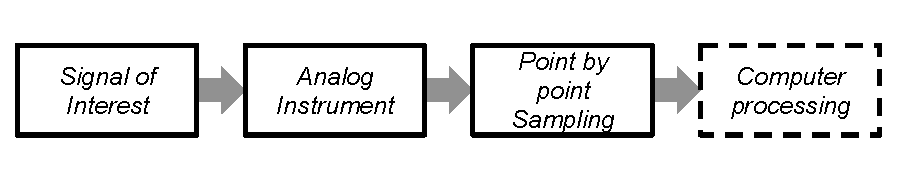
\includegraphics[scale=1]{isomorphicsensorflowchart}
    \caption{A systems view of a traditional sensing scheme. The signal-of-interest is incident upon the analog instrument. The analog instrument forms an isomorphism of the signal which is then periodically sampled point-by-point through an \gls{adc} device. Once the signal is in digital form, post-processing algorithms are often used to perform various tasks such as noise reduction, detection, and classification. Notice that the analog instrument, sampling scheme, and processing are all seperated. }
    \label{fig:isomorphicsesingflowchart}
\end{figure}

We will discuss two important examples of isomorphic sensors: the photographic camera and the optical spectrometer (which I will just call a spectrometer from now on, even though there are many instruments called spectromers that not concerned with optical spectra). These two sensors have had major roles throughout the history of optics and in the physical sciences so it is natural that they have also been the main focus of computational sensing. Therefore it is important we first understand the isomorphic version of these sensors.

In the camera, the signal-of-interest is the object that is being photographed. This can be anything that is scattering or emitting light, a person, a tree or a distant group of stars. The analog instrument consists of the lens which is designed and fabricated to produce an image that is looks like the object at the \gls{fpa}. The more that the image resembles the object the better the optics. The \gls{fpa} then samples and quantizes the image and produces a digital representation of the object, measurement data. The measurement data is often is post-processed to perform such tasks as noise removal or to locate the object. 

There are two major components in the camera which determine how well it performs: the optics and the FPA. Ideally, the optics (the analog instrument in this case) will produce a \gls{psf} which is infinitely small in diameter. For example, in a task such as the detection of a star from several neighboring stars in the night sky, if the \gls{psf} is much larger than the center to center seperation of the two stars in the optical image, it will be quite difficult to detect. A careful reader will note that this is the same argument used by Lord Raleigh in proposing his resolution criterion \cite{rayleigh1879investigations}. Even if the \gls{psf} is small enough, the \gls{fpa} must sample at a fine enough pixel-to-pixel spacing, called the \emph{pixel pitch}, to accurately reproduce the intensity variations at the scale which is pertinant to the task. Intuitively, this makes sense because if the image of both stars and the decreased intensity which signifies a certain amount of seperation between the two stars is imaged onto a single pixel, the one cannot ever hope to be able to accurately the detect the star without some other prior or side information. Shannon, Nyquist, Wittaker and others established the theory for determining what the pixel spacing must be in order to properly sample the analog signal without loosing any information \cite{shannon1949communication, nyquist1924certain, nyquist1928certain}. 

In the spectrometer, the signal of interest is the spectrum of the object. The optics are designed to take the incoming light and seperate various wavelength components. The part of the spectrometer which is used to physically isolate the wavelengths is called a \emph{spectrograph}. The result is a spectral intensity as a function of position at the \gls{fpa}. The \gls{fpa} and post-processing algorithms are used in the same manner as the photographic camera, which is to sample the optical spectrum creating digital version of it and to perform various tasks on the measurement data.
To simplify our discussion, we will concentrate on the slit spectrometer, which spectrum at a single point on the object.

In the spectrometer, one of the important performance metrics is \emph{spectral resolution} which we denote $\delta \lambda$. The spectral resolution is the smallest difference in wavelength the instrument can discern. As in the camera, the optical components plays a major role in determining the spectral resolution. Large spectral resolutions can degrade the spectrometers ability to discern important parts of the spectrum we are testing. Similarly with the camera, the \gls{fpa} must have a pixel pitch which is small enough in order to correctly sample the variations in the spectrum. 

In both the camera and spectrometer, at each exposure, the readout from the \gls{fpa} produces a single number per pixel. The point-by-point sampling of the signal is one of both a strength of isomorphic sensing but is also a source of weakness. 

The strength comes from the straightforward and intuitive architecture of the isomorphic sensor. Each subsystem: the optics, the \gls{fpa}, and the post-processing can be designed and constructed seperately so long as they meet their individual specifications. As long as the \gls{snr} is sufficient and the sampling rate is high enough we are garuenteed to recover the signal.

One of the weaknessess of the isomorphic approach however is the the ability to measure low \gls{snr} signals. Because the image is sampled in a completely parallel fashion at each exposure, each pixel contributes a certain amount of noise (which is independent of the signal strength). If the noise dominates, the measurement fidelity decreases often forcing the operator to incease the exposure time. For weak signals the exposure time can become prohibitive and for temporally dynamic signals this may lead to a loss of resolution. 

It would be easy to assume that with the recent revolution in machine learning and statistical signal processing combined with the dramatic increase in computing power that we could simply post-process poor measurments and obtain useful data. However, this isn't possible due to the an important theorem in information theory called the data processing inequality \cite{cover2012elements}. In layman's term it means "garbage in, garbage out".

Another weakness of isomorhic sensing is that the seperation of the analog instrument, the sampling scheme, and the data processing algorithms lead to increased \gls{swap-c}. As we mentioned in the camera, the optics must be designed to produce a small \gls{psf}. For demanding applications, the optical design and fabrication can be the most expensive component of the sensor. While \gls{fpa} prices in the visible have fallen recently, \glspl{fpa} in certain parts of the electromagnetic spectrum can be quite expensive or non-existant \cite{noor2011compressive}.

In many cases, the signal is redundant and high resolution sampling becomes a waste of resources and data storage. A good example is in photography where often the post-processing takes digital image and applies a compression algorithm which looks for patterns in the signal and reduces the file size, discard much of the sample data \cite{taubman2012jpeg2000}. 

The isomorphic sensor has served humanity well, however with all the weakness that have been discuss I will now begin to discuss some of major techniques that in computational sensing that can be used to address some or all of the issues that I just stated. The first issue is the \gls{snr} and how multiplexing can be used to dramatically reduce exposure times over isomorphic instruments.

\section{Development of Multiplexing in Sensing}


\section{Dissertation Overview}



%\bibliographystyle{IEEEtranS}  
%\bibliography{ThesisBib}

